\documentclass{beamer}
\usetheme{metropolis}           % Use metropolis theme
\setbeamercovered{transparent}

\title{Various pedagogical approaches to classroom teaching}
\date{\today}
\author{Mine \c{C}etinkaya-Rundel}
\institute{Sta 771S - Teaching Statistics}

\begin{document}
\maketitle
 
 
% -------------------------------------------------------------------

\section{Traditional lecture}

% -------------------------------------------------------------------

\begin{frame}
\frametitle{Traditional lecture}

\vfill

What are advantages / disadvantages for lecturing for an entire class period?

\vfill

\end{frame}

% -------------------------------------------------------------------

\begin{frame}
\frametitle{Making your traditional lecture more effective}

\begin{itemize}

\item Structure and organization: Clear learning goals and check points for each lesson

\item Information delivery: Writing on the board, slides, a mix, more...

\item Physical space: Walk around the classroom, use a mic for class size $>$ 40 or so

\end{itemize}

\end{frame}

% -------------------------------------------------------------------

\begin{frame}
\frametitle{Organization: Clear and consistent formatting}

\begin{center}
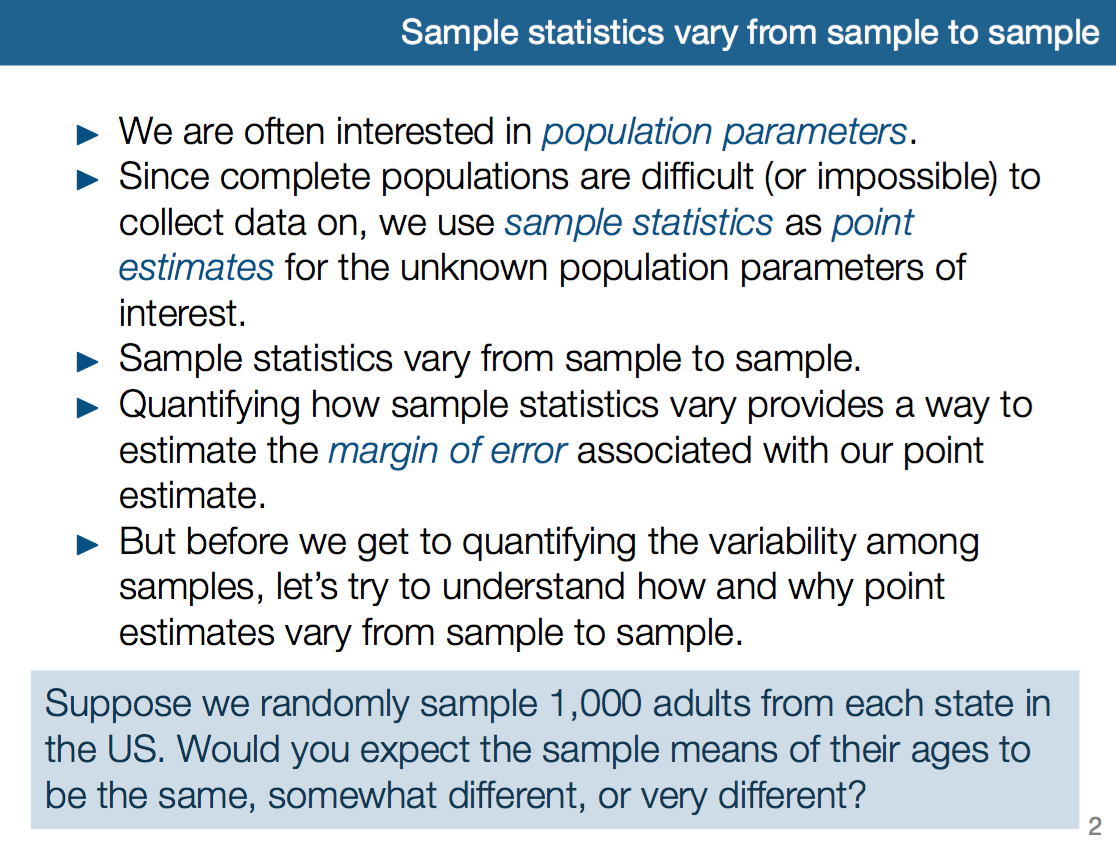
\includegraphics[width = 0.95\textwidth]{figures/disc_question}
\end{center}

\vfill

\end{frame}

% -------------------------------------------------------------------

\begin{frame}[fragile]
\frametitle{Structure: Hide the answers}

If using LaTeX / Beamer, this is easy:

\begin{itemize}

\item For slides you show in class:

\begin{verbatim}
\newcommand{\soln}[1]{\textit{#1}}
\end{verbatim}

\item For slides posted for students:

\begin{verbatim}
\newcommand{\soln}[1]{}
\end{verbatim}

\end{itemize}

\end{frame}

% -------------------------------------------------------------------

\begin{frame}
\frametitle{Make it a little less traditional}

\begin{center}
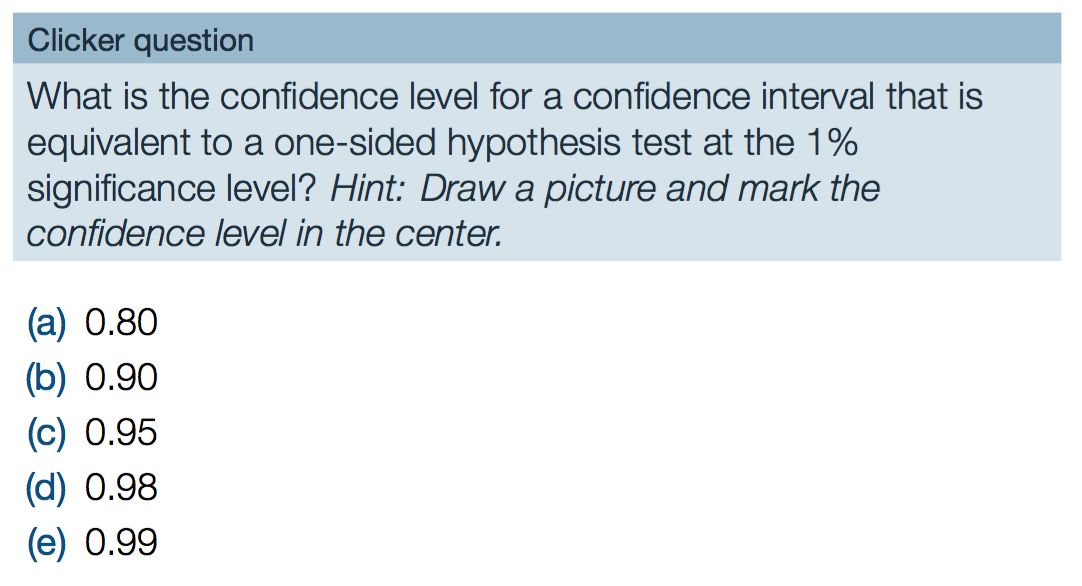
\includegraphics[width = 0.95\textwidth]{figures/clicker_question}
\end{center}

\vfill

\end{frame}

% -------------------------------------------------------------------

\section{Flipped classroom}

% -------------------------------------------------------------------

\begin{frame}
\frametitle{Flipped classroom definition}

The flipped classroom is a pedagogical model in which the typical lecture and 
homework elements of a course are reversed. Short video lectures are viewed 
by students at home before the class session, while in-class time is devoted to 
exercises, projects, or discussions.

\end{frame}

% -------------------------------------------------------------------

\section{Team-based learning (TBL)}

% -------------------------------------------------------------------

\begin{frame}
\frametitle{TBL Definition}

Team-Based Learning is an evidence based collaborative learning teaching strategy 
designed around units of instruction, known as ``modules," that are taught in a three-step cycle: 

\begin{enumerate}
\item preparation
\item in-class readiness assessment
\item application exercises
\end{enumerate}

\begin{center}
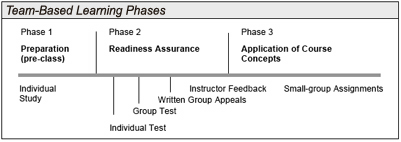
\includegraphics[width = 0.8\textwidth]{figures/TBLPhases}
\end{center}

\end{frame}

% -------------------------------------------------------------------

\begin{frame}
\frametitle{Preparing students for the preparation stage}

\begin{itemize}

\item List of clear learning objectives for the module

\item Textbook reading and/or videos

\item Practice questions

\end{itemize}

\end{frame}

% -------------------------------------------------------------------

\begin{frame}
\frametitle{Readiness assessment}

\begin{itemize}

\item Individual, and then as a Team

\item Delivered via a method that allows the instructor to quickly view results to determine which questions to review

\item Questions should be very clearly tied to learning objectives

\item Good RA design: Average student who studied can get a roughly 80\% individually, and 100\% as a team

\end{itemize}

\end{frame}

% -------------------------------------------------------------------

\begin{frame}
\frametitle{Application exercises}

\begin{center}
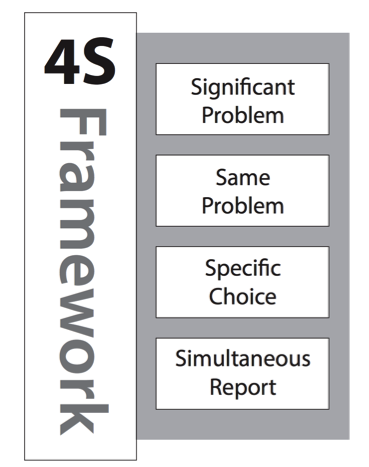
\includegraphics[width = 0.4\textwidth]{figures/4s}
\end{center}

\end{frame}

% -------------------------------------------------------------------

\begin{frame}
\frametitle{Forming teams}

\begin{itemize}

\item Student choice vs. assigned

\item Same team throughout the semester vs. changing

\item Homogenous vs. heterogenous with respect to background in course material

\end{itemize}

\end{frame}

% -------------------------------------------------------------------

\begin{frame}
\frametitle{Challenges for large clases}

\begin{itemize}

\item Need for additional instructor / TA bodies in the class

\item Timing of active components

\item ``Simultaneous reveal" of application exercises

\item Managing team dynamics

\end{itemize}

\end{frame}

% -------------------------------------------------------------------

\section{Hybrid models}

% -------------------------------------------------------------------

\begin{frame}
\frametitle{Hybrid models}

\vfill

Don't feel like you have to limit yourself to the strict definition of a specific pedagogy

\vfill

Think about how you can borrow ideas from various pedagogies to make the most of your course

\end{frame}


% -------------------------------------------------------------------

\begin{frame}{Sta 101}
\frametitle{}

\begin{itemize}

\item Course is divided into seven learning units. 

\item Each unit has a set of learning objectives and required and suggested readings, videos, etc. Students are expected to watch the videos and/or complete the readings and familiarize themselves with the learning objectives. 

\item Begin the unit with a readiness assessment: 10 multiple choice questions that you answer using clickers and then re-take in teams using scratch off sheets.

\item Rest of the class split between discussion of the material and application exercises completed in teams. All class materials posted on course website.

\item Within each unit complement learning with problem sets and labs.

\item Wrap up each unit with a performance assessment.

\end{itemize}

\end{frame}

% -------------------------------------------------------------------

\section{Regardless of pedagogy}

% -------------------------------------------------------------------

\begin{frame}
\frametitle{Regardless of pedagogy}

you should have a

\begin{itemize}

\item detailed syllabus that clearly outlines all expectations and course logistics

\item a well organized course website (better -- for you -- if some components are public!) 

\end{itemize}

\end{frame}

% -------------------------------------------------------------------

\section{Visit a class}

% -------------------------------------------------------------------

\begin{frame}
\frametitle{}

\vfill

Visit one (or more) classes (not lab session) between now and March 22.

\vfill

You're welcomed to visit my class: MW 1:25 - 2:40pm, see \href{http://bitly.com/sta101\_s16}{http://bitly.com/sta101\_s16} for schedule (avoid exam days)

\vfill

\end{frame}

% -------------------------------------------------------------------




\end{document}